\section{Introduction}
Recent advancements, represented by models like DeepSeek-R1 \citep{guo2025deepseek}, mark a paradigm shift towards ``slow thinking''. 
By leveraging Reinforcement Learning (RL) to encourage extended Chains of Thought (CoT), these models have achieved remarkable breakthroughs in complex reasoning tasks. 
However, a critical paradox has emerged: while scaling reasoning compute significantly boosts problem-solving abilities, it does not naturally align with factual reliability. 
In fact, slow thinking models often exhibit severe hallucinations \citep{heyman2025reasoning,patel2024multi,arcuschin2025chain}. 
As shown in Figure~\ref{fig:scaling}, larger reasoning models achieve higher GPQA~\citep{rein2024gpqa} scores but fail to improve or even regress on hallucination benchmarks like SimpleQA \citep{wei2024measuring}. 
For instance, the DeepSeek-R1-Distill-Qwen-32B \citep{guo2025deepseek} achieves an accuracy of only 6.64\% on the SimpleQA dataset. 
This suggests that without proper guidance, the long reasoning process can turn into a "snowball" of errors, where one small mistake leads to a completely fabricated conclusion. 
This raises a critical question: \textit{\textbf{Why do models with such strong reasoning abilities still fail so badly at factual reliability?}}

% DeepSeek-R1 \citep{guo2025deepseek} demonstrates that through meticulously designed reward functions, Reinforcement Learning (RL) can significantly enhance the reasoning ability of models. 
% Slow-thinking models often exhibit severe hallucinations, particularly during extended chains of thought or complex reasoning processes, where initial inaccuracies can become significantly amplified. 
% This vulnerability is highlighted by the performance of even large-scale models; for instance, the DeepSeek-R1-Distill-Qwen-32B \citep{guo2025deepseek} achieves an accuracy of only 6.64\% on the SimpleQA \citep{wei2024measuring} dataset.

% \begin{figure}[t!]
%     \centering
%     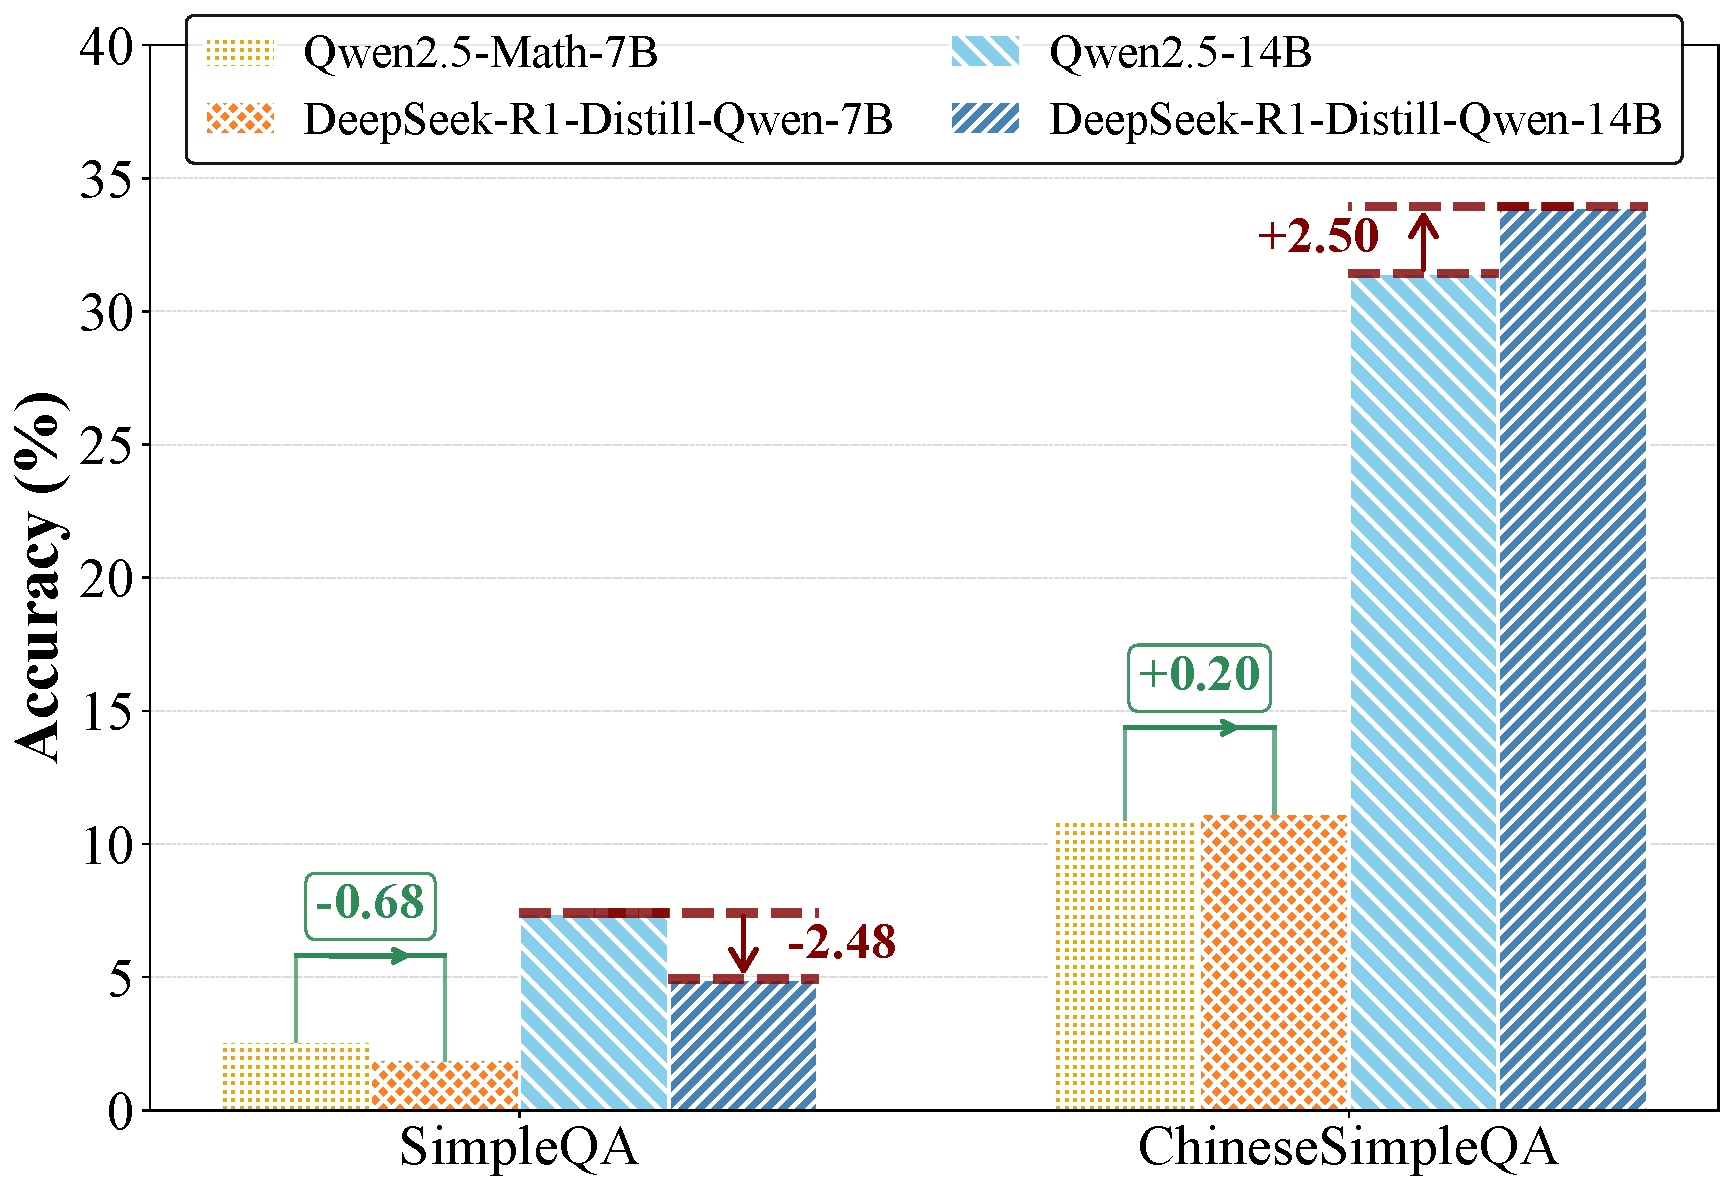
\includegraphics[width=\columnwidth]{images/model-comparison-barchart.pdf}
%     % \vspace{-2ex}
%     \caption{Performance of all models on SimpleQA and ChineseSimpleQA.}
%     \vspace{-3ex}
%     \label{slow-thinking-hallucination}
% \end{figure}
\begin{figure}[t!]
    \centering
    \resizebox{.45\textwidth}{!}{
    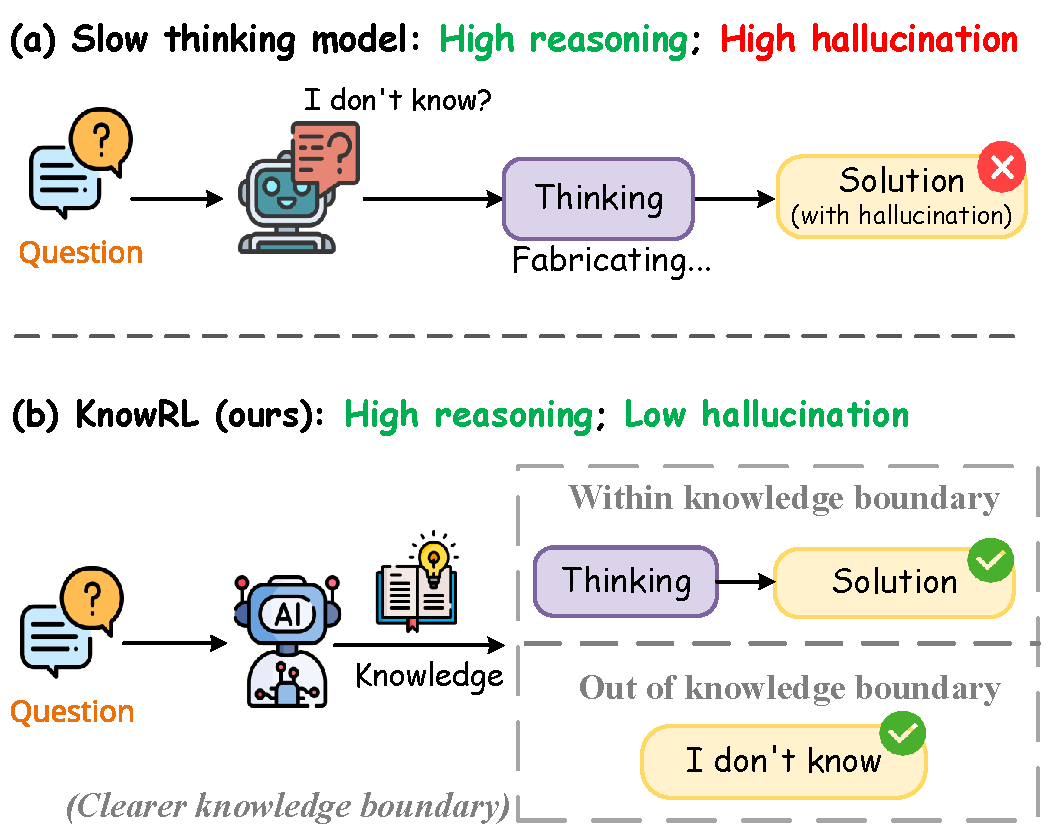
\includegraphics{images/intro.pdf}}
    \caption{KnowRL reduces hallucinations in slow-thinking models.}
     \vspace{-3ex}
    \label{fig:intro}
\end{figure}

The root cause lies in the way we currently train these models.
Standard RL heavily relies on outcome-oriented rewards, which optimize for the final answer while treating the reasoning process as a black box. 
This approach has two main flaws.
\textit{First}, it ignores the Knowledge Boundary---the model's ability to distinguish between what it knows and what it does not know. 
Without this boundary, models try to guess the answer to get the reward. 
\textit{Second}, it creates a supervision gap: model might generate a correct answer using wrong or made up reasoning steps. 
Since the reward signal depends solely on the final outcome, the model mistakenly learns that fabricating reasoning paths is a valid strategy; therefore, the RL algorithm unwittingly reinforces this hallucinated logic.
Consequently, the model becomes ``smart'' at reasoning but ``dishonest'' about facts.

Addressing this challenge with existing methods proves difficult. 
Retrieval Augmented Generation \citep[RAG;][]{lewis2020retrieval} faces significant retrieval efficiency bottlenecks when integrated into the extensive reasoning steps of slow thinking models. 
Supervised Fine Tuning \citep[SFT;][]{ouyang2022training} primarily relies on static knowledge injection. 
However, this paradigm suffers from severe catastrophic forgetting \citep{chen2025retaining}, often degrading the model's inherent reasoning capabilities. 
More fundamentally, SFT encourages the model to merely memorize static knowledge rather than learning the generalized behavior of reasoning.
Consequently, it fails to instill the critical strategy of ``knowing what you know and what you do not know''---a dynamic judgment of Knowledge Boundaries. 
In contrast, Reinforcement Learning is uniquely suited to shape this behavioral strategy \citep{gandhi2025cognitive}.
Therefore, there is an urgent need for a RL framework that can inherently instill factual discipline into the model's reasoning behaviors without compromising its reasoning capabilities.




% RL driven by outcome rewards often neglects the LLM's reasoning process, leading to correct outputs from flawed internal reasoning. 
% Generalizing such incorrect reasoning patterns significantly increases hallucination risk. 
% This issue is exacerbated in slow-thinking models trained via RL on mixed task types, partly because simple open-domain factual tasks and complex reasoning tasks (e.g., mathematics) have differing training requirements. 
% Fundamentally, models lacking factual guidance during training may resort to any means to obtain rewards, resulting in highly unreliable thinking processes. 
% Existing hallucination mitigation methods have limitations: Supervised Fine-Tuning \citep[SFT;][]{ouyang2022training} with high-quality data is costly and difficult to scale; Retrieval Augmented Generation \citep[RAG;][]{lewis2020retrieval} encounters efficiency and fusion challenges in long Chain-of-Thought (CoT) reasoning; and decoding-stage interventions \citep{chuang2023dola} can disrupt strategies learned through RL. 
% Crucially, these approaches do not consistently preserve strong reasoning capabilities while reducing hallucinations. 
% Therefore, a more reliable method involves introducing knowledge to supervise the model's thinking process during RL training.
\begin{figure}[t]
    \centering
    \resizebox{.45\textwidth}{!}{
    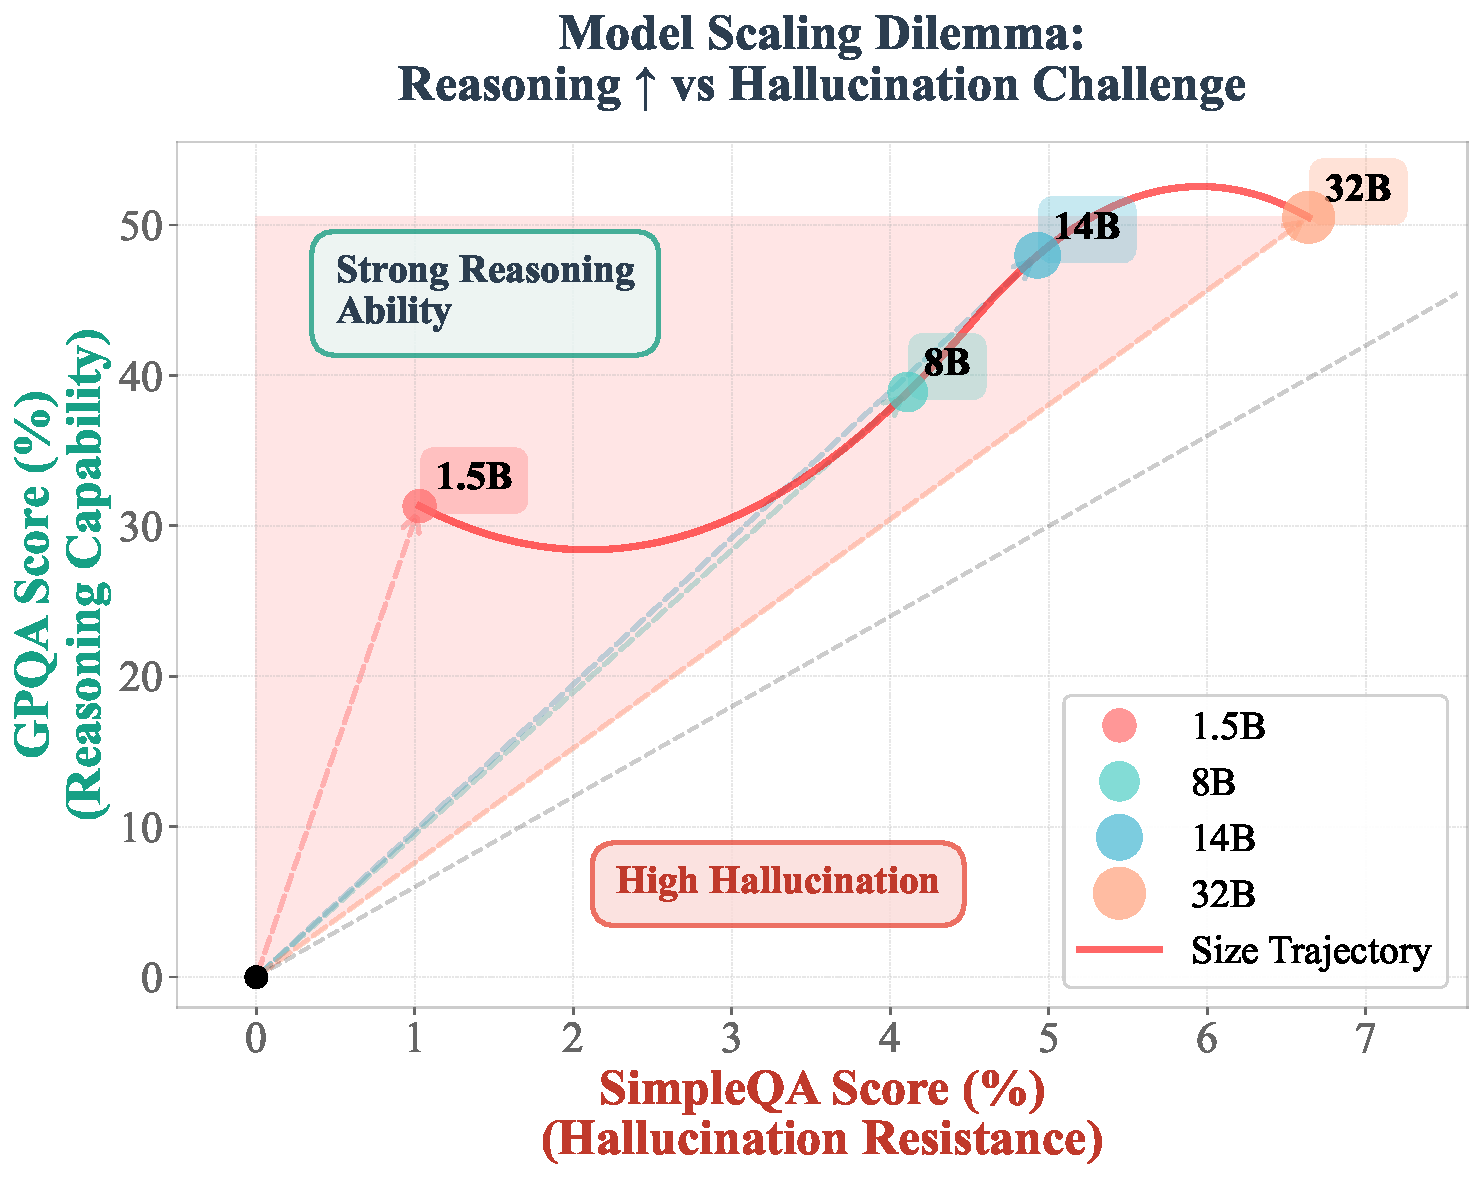
\includegraphics{images/model_scaling_analysis.pdf}}
    \caption{Scaling improves reasoning ability (GPQA) but does not reduce hallucinations (SimpleQA). Results are shown for DeepSeek-R1-Distill models of varying sizes (Qwen-1.5B, Llama-8B, Qwen-14B, Qwen-32B).}
    \vspace{-3ex}
    \label{fig:scaling}
\end{figure}

So, to bridge this gap, we propose Knowledge enhanced Reinforcement Learning (KnowRL), a framework that integrates factuality supervision directly into the RL reasoning loop. 
Unlike outcome-based approaches, KnowRL opens the ``black box'' of thinking. 
By decomposing the Chain of Thought into atomic facts and verifying them against the corresponding ground-truth knowledge, KnowRL provides dense, process level rewards. 
This design transforms the RL objective: instead of merely ``getting the answer right,'' the model is incentivized to reason faithfully and, crucially, to recognize its knowledge boundaries---learning to say ``I don't know'' rather than fabricating a plausible sounding response when information is missing, as illustrated in Figure~\ref{fig:intro}.

Experimental results validate the effectiveness of KnowRL. 
On hallucination benchmarks, KnowRL significantly reduces the error rate. 
For instance, dropping the Incorrect Rate on SimpleQA by 20.3\% for 7B slow thinking model. 
Crucially, this gain in factuality does not come at the cost of reasoning ability; KnowRL maintains strong performance on complex reasoning datasets like GPQA and AIME 2025. 
Furthermore, our method demonstrates strong transferability and Out-Of-Distribution (OOD) generalization to knowledge domains outside the training distribution; it significantly improves performance on ChineseSimpleQA~\citep{he2024chinese} even when the primary knowledge source is purely English-based. 
These findings suggest that KnowRL helps the model internalize a universal verification behavior rather than merely memorizing language-specific facts.  
These results confirm that KnowRL successfully aligns the slow thinking process with factual accuracy, offering a robust path for building reliable reasoning models.

% To address this, we propose Knowledge-enhanced Reinforcement Learning (KnowRL), a method that integrates a factuality reward into the RL training process. This reward, inspired by FactScore \citep{min2023factscore} and obtained by evaluating textual support against an external knowledge base, guides the model to perform fact-based slow thinking. 
% KnowRL cooperatively optimizes reasoning and fact-following in slow-thinking models by helping them learn better knowledge boundaries to avoid fabricating facts, as illustrated in Figure~\ref{fig:intro}. 
% Our extensive experiments validate KnowRL's significant impact. 
% Across benchmarks such as TruthfulQA~\citep{lin2021truthfulqa}, KnowRL consistently mitigates hallucinations while preserving reasoning ability. For distillation-based slow-thinking models, KnowRL training reduces the error rate on SimpleQA by 20.3\%, while maintaining strong reasoning performance on GPQA~\citep{rein2024gpqa} and AIME 2025. Moreover, KnowRL substantially decreases incorrect responses on ChineseSimpleQA~\citep{he2024chinese}, a dataset outside our English-based knowledge source, demonstrating that KnowRL learns transferable knowledge boundaries and improves factual reliability beyond the original knowledge base.




% The main contributions of this paper are as follows:
% \begin{itemize}
%     \item We introduce KnowRL, a novel framework using factuality rewards from external knowledge to reduce hallucinations in LLMs while preserving their reasoning ability.
%     \item We demonstrate through comprehensive experiments that KnowRL effectively mitigates hallucinations and maintains reasoning in diverse slow-thinking models.
%     \item We contribute a carefully constructed, high-quality training dataset for factual tasks, crucial for initializing and training KnowRL.
% \end{itemize}

% \begin{itemize}
%     \item We propose KnowRL, a Reinforcement Learning framework using factuality rewards from knowledge verification to reduce slow-thinking model hallucinations while maintaining strong reasoning ability.
%     % \item Our experiments identify optimal KnowRL training configurations: essential cold-start SFT for factuality reward efficacy, and balanced cold-start data volume and RL training duration to mitigate hallucinations without impairing reasoning or causing overtraining.
%     \item Our experimental analyses identify key training configurations for KnowRL's efficacy: foundational cold-start SFT is essential for activating factuality rewards, while optimal cold-start data volume and RL training duration are crucial to balance hallucination mitigation with reasoning ability, preventing negative impacts from suboptimal data quantities or overtraining.
%     \item We constructed high-quality reasoning training datasets for open-domain factual tasks and distilled high-quality SFT long COT datasets for factual tasks.
% \end{itemize}




